% ---------------------------------------------------------------------
% 2.1 skyrius. Analizės klasių diagrama
% Naudojimas pagrindiniame dokumente:   \input{analizes-klasiu-diagrama}
% Reikalingi paketai: graphicx, booktabs, longtable, array, caption
% Paveikslėlis: diagramos/analizes-klasiu-diagrama.png
% (iš .puml: java -jar plantuml.jar -charset UTF-8 -tpng diagramos/*.puml)
% ---------------------------------------------------------------------

\subsection{Analizės klasių diagrama}
\label{sec:analizes-klasiu-diagrama}

Analizės klasių diagrama (\ref{fig:analizes-klasiu-diagrama} pav.) parodo sistemos
dalykinės srities sąvokas, jų savybes, pagrindines atsakomybes ir ryšius. Esybių klasės
atitinka ER diagramos esybes ir panaudojimo atvejų
analizėje suderintus terminus: naudotojo paskyra, dalyvio profilis, trenerio profilis,
sporto erdvė, įrenginys, pratimas, mokomoji medžiaga, užsiėmimo programa ir jos versija,
programos etapas, užsiėmimas, rezervacija, lankomumo įrašas, asmeninė programa,
įvertinimas, pasiruošimo rekomendacija, namų užduotis ir vykdymo žurnalas.

Diagramoje laikomasi šių sprendimų:
\begin{itemize}
  \item Vietinis grotuvas, vidinis laikmatis ir virtualaus trenerio režimas nėra atskiros
        esybių klasės: virtualaus trenerio užsiėmimas pažymimas užsiėmimo atributu
        \emph{režimas}, o tuščias \emph{treneris} nurodo virtualų trenerį.
  \item Vaidmenys (dalyvis, treneris, administratorius) išreikšti naudotojo paskyros
        atributu \emph{vaidmuo}; administratorius profilio neturi.
  \item Dalyvis su treneriu susiejamas tik per rezervaciją, nuolatinio priskyrimo
        klasės nėra.
  \item Lankomumo įrašas susietas su rezervacija; žymos nebuvimas reiškia, kad
        lankomumas nepažymėtas, o ne „nedalyvavo“.
  \item Ryšių kardinalumas žymimas pagal \ref{tab:er-zymejimas} lentelę.
\end{itemize}

\begin{figure}[H]
  \centering
  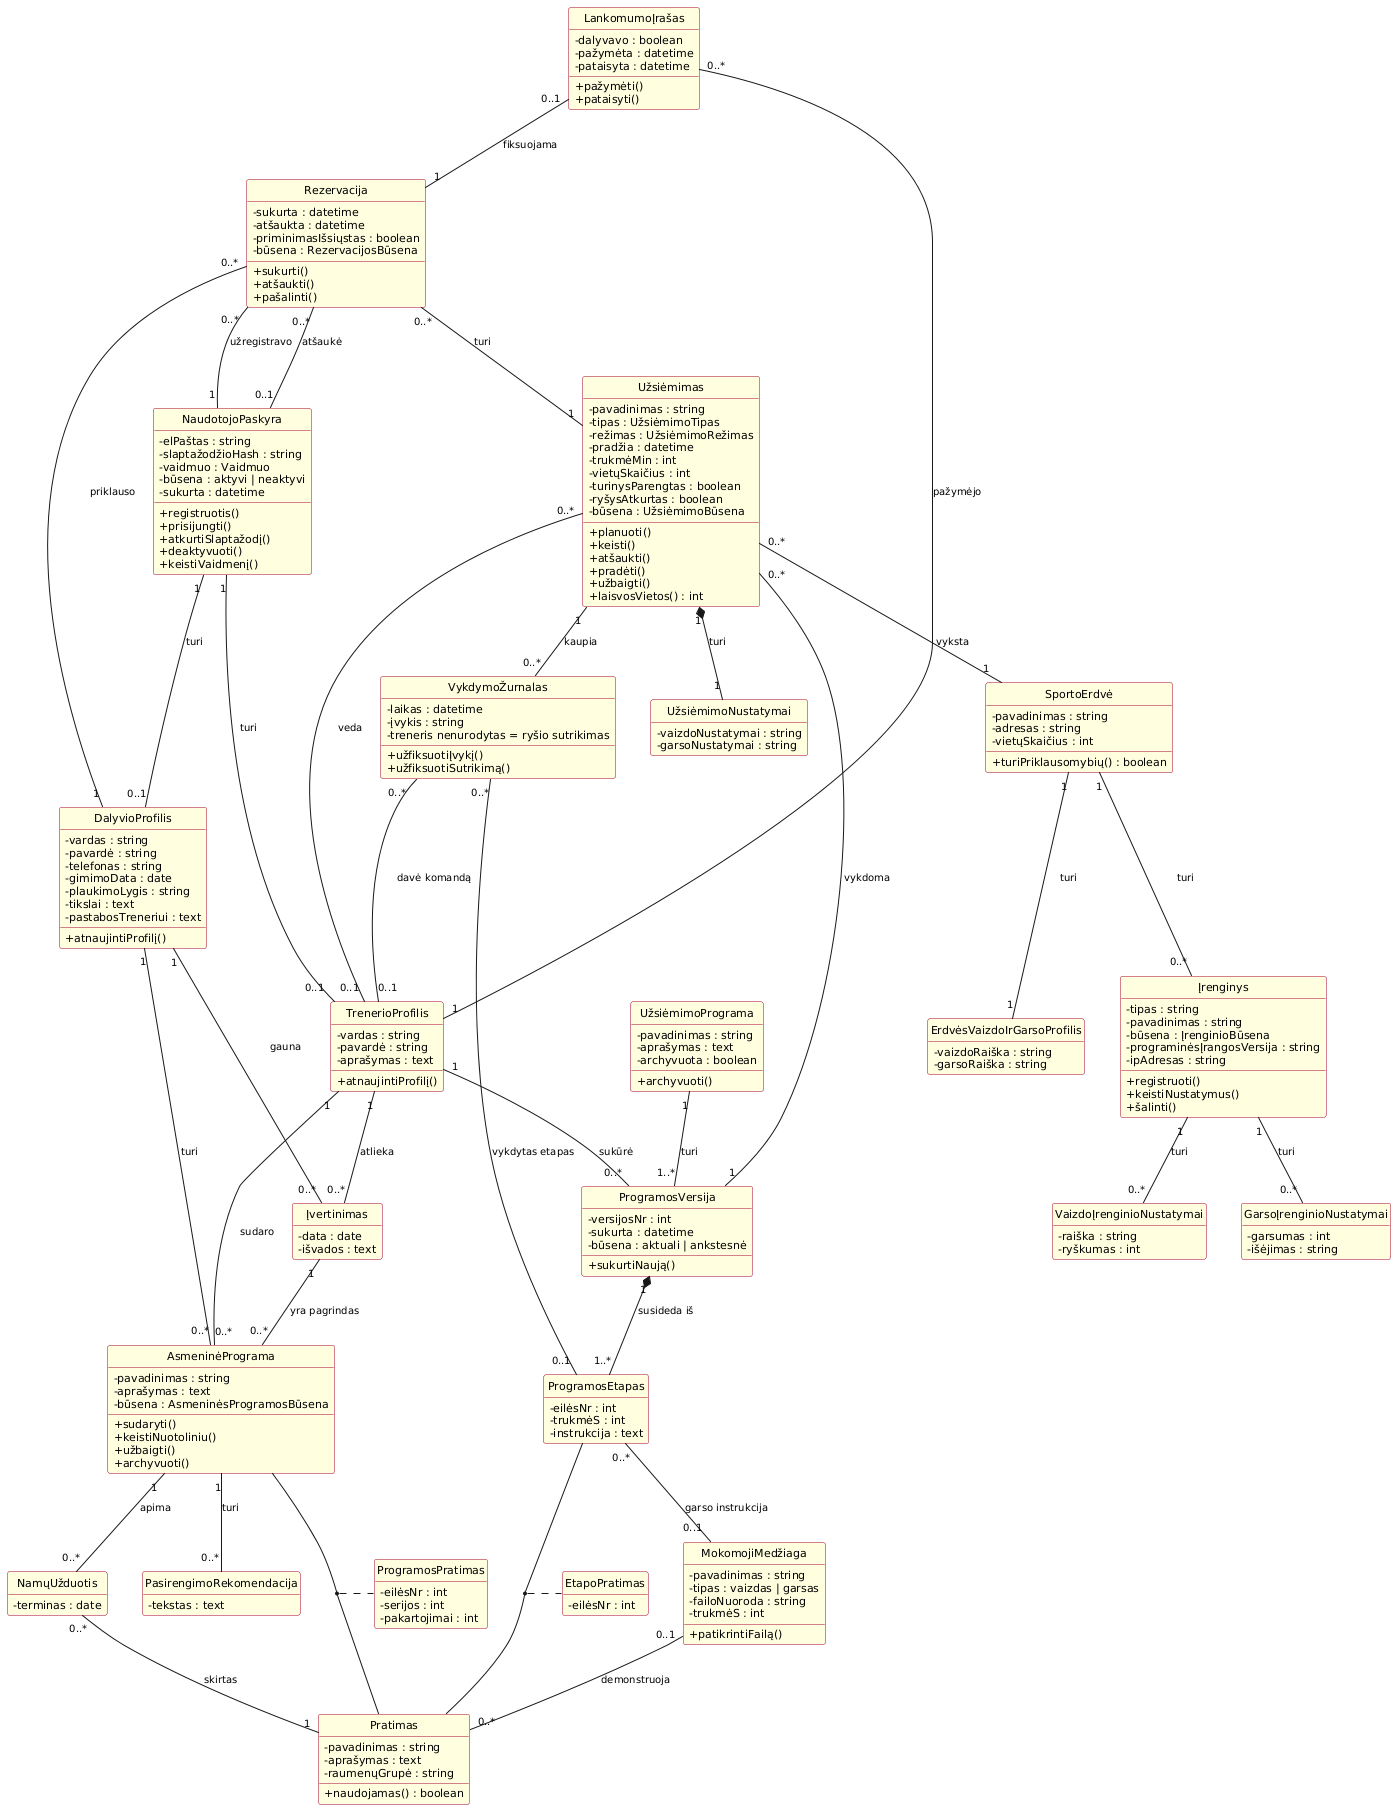
\includegraphics[width=\textwidth,height=0.88\textheight,keepaspectratio]{OOA analizė/Analizės klasių diagrama/analizes-klasiu-diagrama.png}
  \caption{Analizės klasių diagrama}
  \label{fig:analizes-klasiu-diagrama}
\end{figure}

\paragraph{Klasių aprašai.}

\begin{longtable}{@{}p{0.27\textwidth}p{0.45\textwidth}p{0.20\textwidth}@{}}
\caption{Analizės esybių klasės ir jų atsakomybės}\label{tab:analizes-klases}\\
\toprule
\textbf{Klasė} & \textbf{Atsakomybė} & \textbf{PA} \\
\midrule
\endfirsthead
\toprule
\textbf{Klasė} & \textbf{Atsakomybė} & \textbf{PA} \\
\midrule
\endhead
\bottomrule
\endfoot
NaudotojoPaskyra & Prisijungimo duomenys, vaidmuo ir paskyros būsena (aktyvi, neaktyvi) & PA-01, PA-02 \\
DalyvioProfilis & Dalyvio asmens duomenys, plaukimo lygis, tikslai ir pastabos treneriui & PA-01, PA-13 \\
TrenerioProfilis & Trenerio duomenys; treneris kuria programas, veda užsiėmimus ir žymi lankomumą & PA-05, PA-06 \\
SportoErdvė & Erdvės pavadinimas, adresas ir vietų skaičius; šalinimas blokuojamas esant priklausomybių & PA-03 \\
ErdvėsVaizdoIrGarsoProfilis & Erdvei skirta vaizdo ir garso raiška & PA-03 \\
Įrenginys & Erdvėje registruojama įranga, jos būsena (naudojamas, taisomas, grąžintas) ir programinės įrangos versija & PA-03 \\
VaizdoĮrenginioNustatymai, GarsoĮrenginioNustatymai & Įrenginio vaizdo (raiška, ryškumas) ir garso (garsumas, išėjimas) nustatymai & PA-03 \\
Pratimas & Pratimo pavadinimas, aprašymas ir raumenų grupė; susietas su demonstracine medžiaga; naudojamas pratimas nešalinamas & PA-04 \\
MokomojiMedžiaga & Patvirtintas vaizdo ar garso failas (Full HD riba) su metaduomenimis & PA-04 \\
UžsiėmimoPrograma & Programos pavadinimas ir aprašymas; naudojama programa archyvuojama, ne šalinama & PA-05 \\
ProgramosVersija & Nekeičiama programos versija; viena versija aktuali, ankstesnės lieka istorijoje & PA-05 \\
ProgramosEtapas & Etapo eilė, trukmė ir instrukcija; susieja pratimus (per EtapoPratimas) ir garso instrukcijos medžiagą & PA-05, PA-15 \\
Užsiėmimas & Suplanuotas individualus ar grupinis užsiėmimas (su treneriu arba virtualus): laikas, erdvė, programos versija, vietos, būsena & PA-06--PA-08, PA-15 \\
UžsiėmimoNustatymai & Užsiėmimo vaizdo ir garso nustatymai & PA-15 \\
Rezervacija & Dalyvio vieta užsiėmime (aktyvi, atšaukta, pašalinta), kas ją sukūrė ar atšaukė, priminimo žyma & PA-09--PA-11, PA-18 \\
LankomumoĮrašas & Faktinis dalyvavimas (dalyvavo / nedalyvavo), kas ir kada pažymėjo ar pataisė & PA-12, PA-17 \\
VykdymoŽurnalas & Užsiėmimo vykdymo įvykiai ir ryšio sutrikimai (be trenerio -- sutrikimas) & PA-15, PA-16 \\
Įvertinimas & Individualus trenerio atliktas dalyvio įvertinimas, pagrindžiantis asmeninę programą & PA-13 \\
AsmeninėPrograma & Dalyviui sudaryta programa (galiojanti, užbaigta, archyvuota), keičiama nuotoliniu būdu & PA-13, PA-14 \\
ProgramosPratimas & Asmeninės programos pratimas su eile, serijomis ir pakartojimais & PA-13, PA-14 \\
NamųUžduotis & Dalyviui skirta užduotis, susieta su pratimu ir terminu & PA-13, PA-14 \\
PasirengimoRekomendacija & Rekomendacijos tekstas asmeninei programai & PA-13, PA-14 \\
\end{longtable}
